\section{Evaluation}
\label{sec:result}
% use one net to represent a complicated scene
% we still have other option for real-time, like streaming
\note{
Ablation studies for the network training/losses
Target scene | uniformly downsampled image | local foveated rendered image | network predicted images ---> at least 4 different scenes.
streaming time for 4-5 different scenes: full resolution vs our network prediction for “same data size”
image quality of rendered scene vs our network prediction for “same amount of streaming time”
User study results
Table on performance comparison, streaming time, PSNR, SSIM, etc
}%note
\subsection{User Study}
\label{sec:study:user}
% \zh{(Jan 10) all the Qs are answered offline, will update the section soon.}

% In this section, we report two perceptual experiments to investigate 1) how users perceive our solution and the ground truth and 2) how our solutions behaves compared to other alternatives.
In this section, we report a perceptual experiment to investigate how users perceive our solution compared to the ground truth and state-of-the-art (we choose to apply NeRF on our dataset).

% \zh{usually we report the study design here too, like within-subject user study and analyze method, like ANOVA. But I am not sure what we should use here.}
% \zh{(Jan 12), if we include NeRF, I'd say we keep one of the down-sample conditions}

\paragraph{Stimuli}
We designed four conditions for the perceptual experiment (see \autoref{fig:results:comparison}). The first column is the target scene, which we treat as the ground truth. The size of the image per eye is 1440 x 1600. The second column is a uniformly down-sample image at size \warning{??? x ???}. Assuming our network bandwidth is \warning{???}, to stream the images from the cloud in real time, the largest size of the image per eye is up to \warning{??? = ??? / 50 fps / 2 eyes}. So we down sample the entire image with ratio \warning{???}.
% The third column enables foveated rendering. The foveated area is preserved as the original resolution while the rest of the image is down sampled. We apply the same alpha blending method that we used in our solution (see \autoref{sec:method:blending}). Similarly, we calculate the size of the foveated image based on the bandwidth. Hence the down-sample ratio of peripheral area is \warning{???}. 
The fourth column is generated by NeRF implementation. We assign $N_{sample}=16$. The last column is our result. We predict the image from the camera transformation, fine-tune the foveated layer with local guided view, and render the image by alpha blending the three layers. The duration of the stimuli was \warning{??} seconds for each condition. 
% \zh{unsure if we want to render real-time results according to users gaze movement, or show static images with predefined gaze positions for certain duration?}

\paragraph{Setup}
?? users (\warning{? females and ? males, $M=?$, $SD=?$}) participated in the study. They were not involved in the project previously. Each participant was asked to wear a HTC Vive Pro Eye headset during the experiment.  During the experiment, the participants wearing the headset explored our stimuli. We used the \textit{two-alternative forced choice} (2AFC) method for both of our studies. 

\paragraph{Task}
The task was a two-alternative-forced-choice (2AFC). 
Each participant were provided with \warning{30?} trials where each trial consisted a foveated area indicator and a pair of two stimuli. We randomize the order of the pairs for counterbalancing. To control the images to be shown for each participant, we choose to render the results for all conditions on predefined gaze positions rather than passing user's real time gaze input to the system. We indicate the location of the foveated area to users in advance to all the conditions first. For each condition, participants were instructed to indicate which of the two conditions appeared to be with higher quality. 

% \zh{Since we will show at least four conditions to each participant, are we gonna ask them to pick up ONE as the favorite or ask them to judge each condition as ACCEPTED or NOT ACCEPTED? Or we should apply 3 trials that each contains ours and one of other alternatives? For example, Condition1 v.s. ConditionOurs, Condition2 v.s. ConditionOurs, and Condition3 v.s. ConditionOurs}
To minimize the effect of accumulating discomfort during the experiment, we enforced at least a 60-second break between the two conditions in each trial, but the participants were instructed to take as much time as needed to recover.
% \zh{I think rendering static images rather than taking real gaze input is more controllable and good for comparison, because we cannot control users gaze input, thus the images shown to participants are not the same. If we wanna follow a within subject study design, we probably need to pre-generated the gaze path. HOWEVER, if it does not matter if the participants need to look at the same images, which means the study is not ``paired'', we can still take real gaze input. But I think it increases the pressure for implementation, and we are not designing a gaze tracking system actually. How do you think about it?}


%\qisun{Here is what I think. The conditions, OURS, UNIFORM (i.e. downsampled), NERF could be described in the stimuli part. Then in the task paragraph, we simply compare any given pair of these 3 conditions.}
% \zh{no more down samples?}
%\zh{no GT included?}

\paragraph{Results and discussion}
\Cref{fig:results:2afc} plots the study results. 

\begin{figure}[htb]
    \centering
    \includegraphics[width=0.96\linewidth]{example-image-a}
    \caption{The users' preference votes from our evaluation experiment.}
    \label{fig:results:2afc}
\end{figure}

% apply binomial test https://docs.scipy.org/doc/scipy/reference/generated/scipy.stats.binom_test.html
% or apply ANOVA, there is a value of votes for each condition and we want to know if there exists significant effects on different condition.

The results about indicated the similar perceptual quality between {\bf OURS} and {\bf GT}. However, the participants significantly observed the quality drop from {\bf NERF}. 

To further validate the perceptual quality, we conducted measurements with objective metrics in the following section.

\subsection{Visual Quality}
As a complementary to the subjective measurement \Cref{sec:study:user}, we evaluate the perceived quality in an objective fashion. Specifically, we compare our method with both full resolution rendering and \cite{mildenhall2020nerf} with the same time consumption.

\begin{figure}
    \centering
    \subfloat[ANOVA on FWQI]{\includegraphics[width = 0.8\linewidth]{example-image-a}}

    \subfloat[FWQI gaze heatmap]{\includegraphics[width = 0.8\linewidth]{example-image-a}}
    \caption{Objective measurements on visual quality.}
    \label{fig:result:visual}
\end{figure}

\begin{figure*}[htb]
    \centering
    \begin{minipage}{0.32\linewidth} %full res
        \subfloat[]{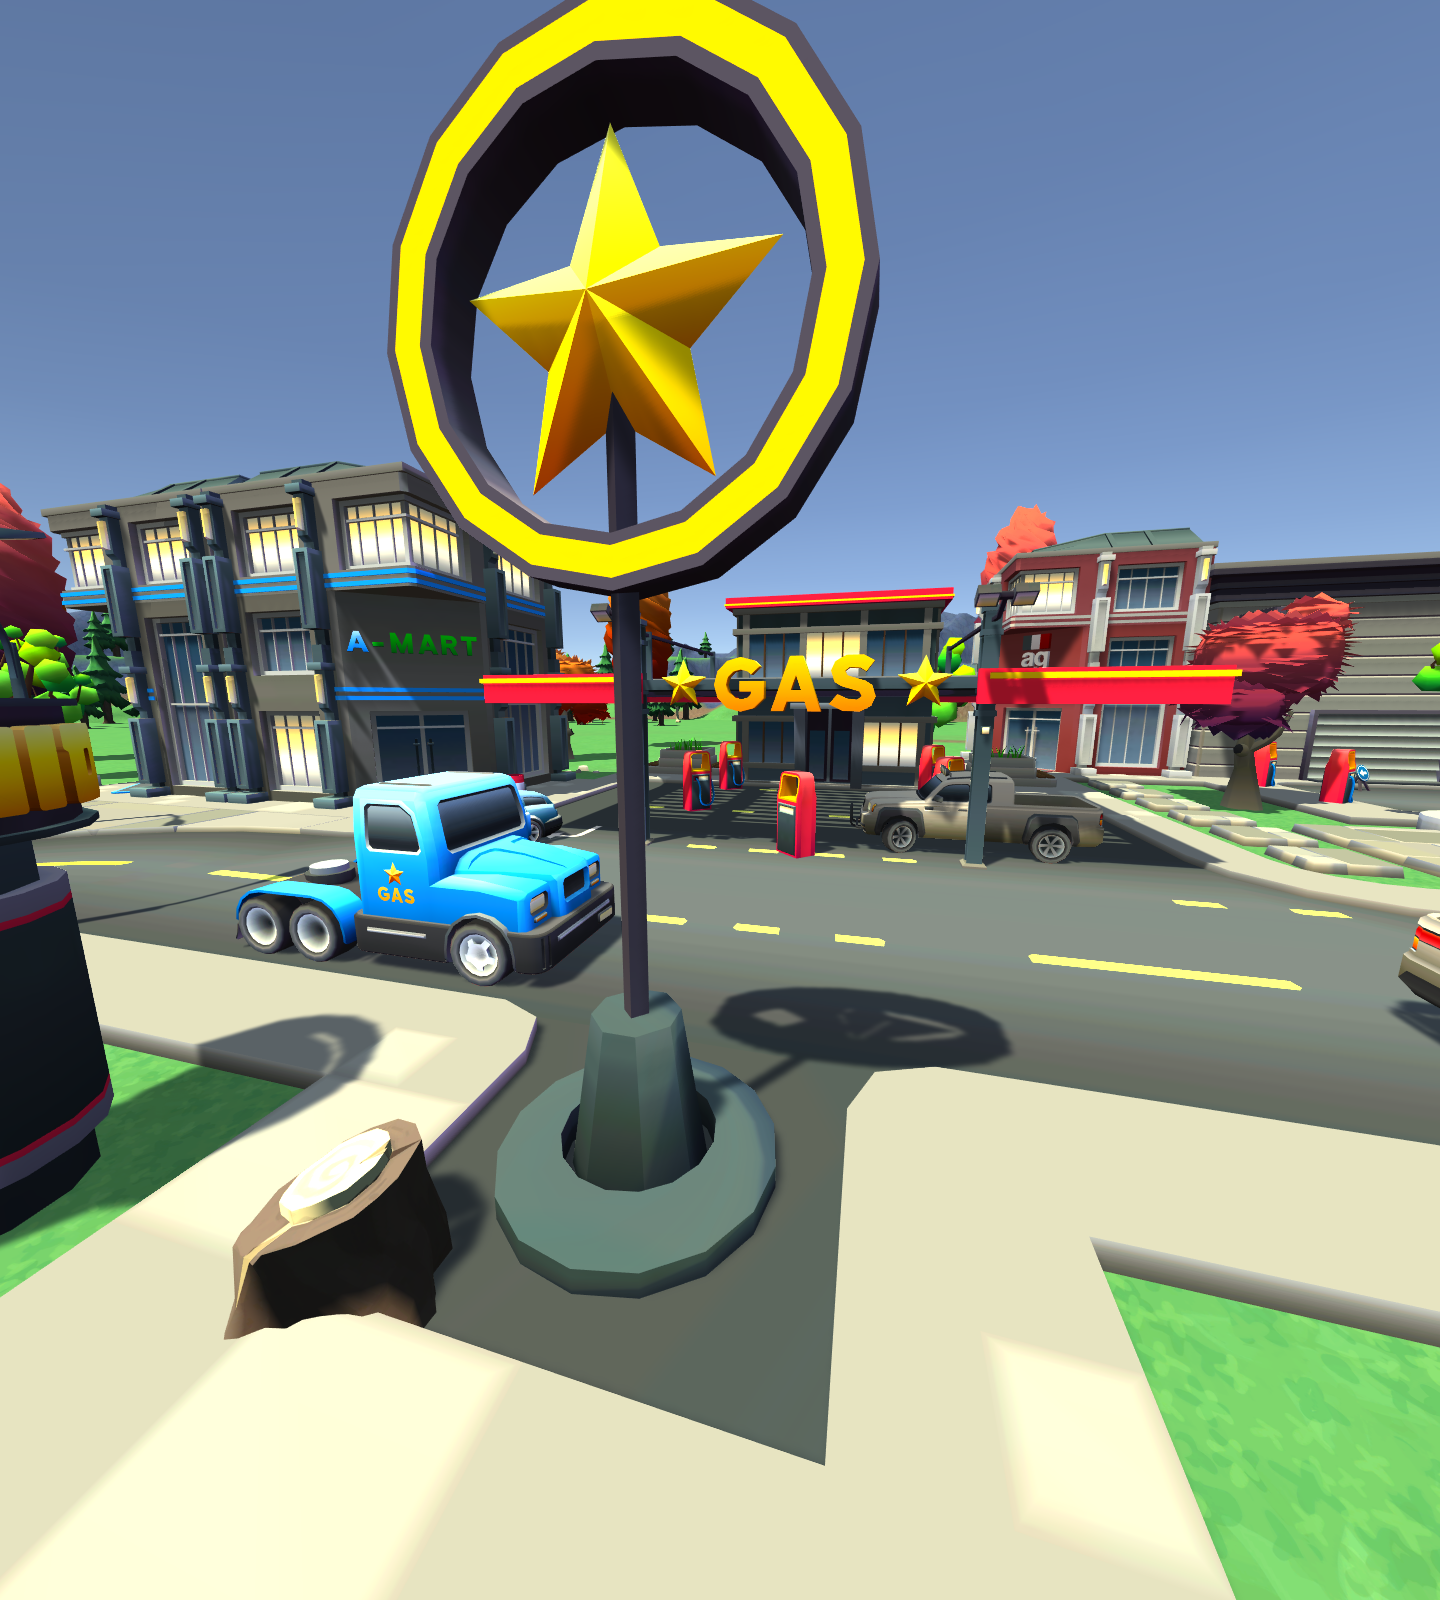
\includegraphics[width=0.96\linewidth]{TOG/figs/gas_gt4.png}}
        
        \subfloat[]{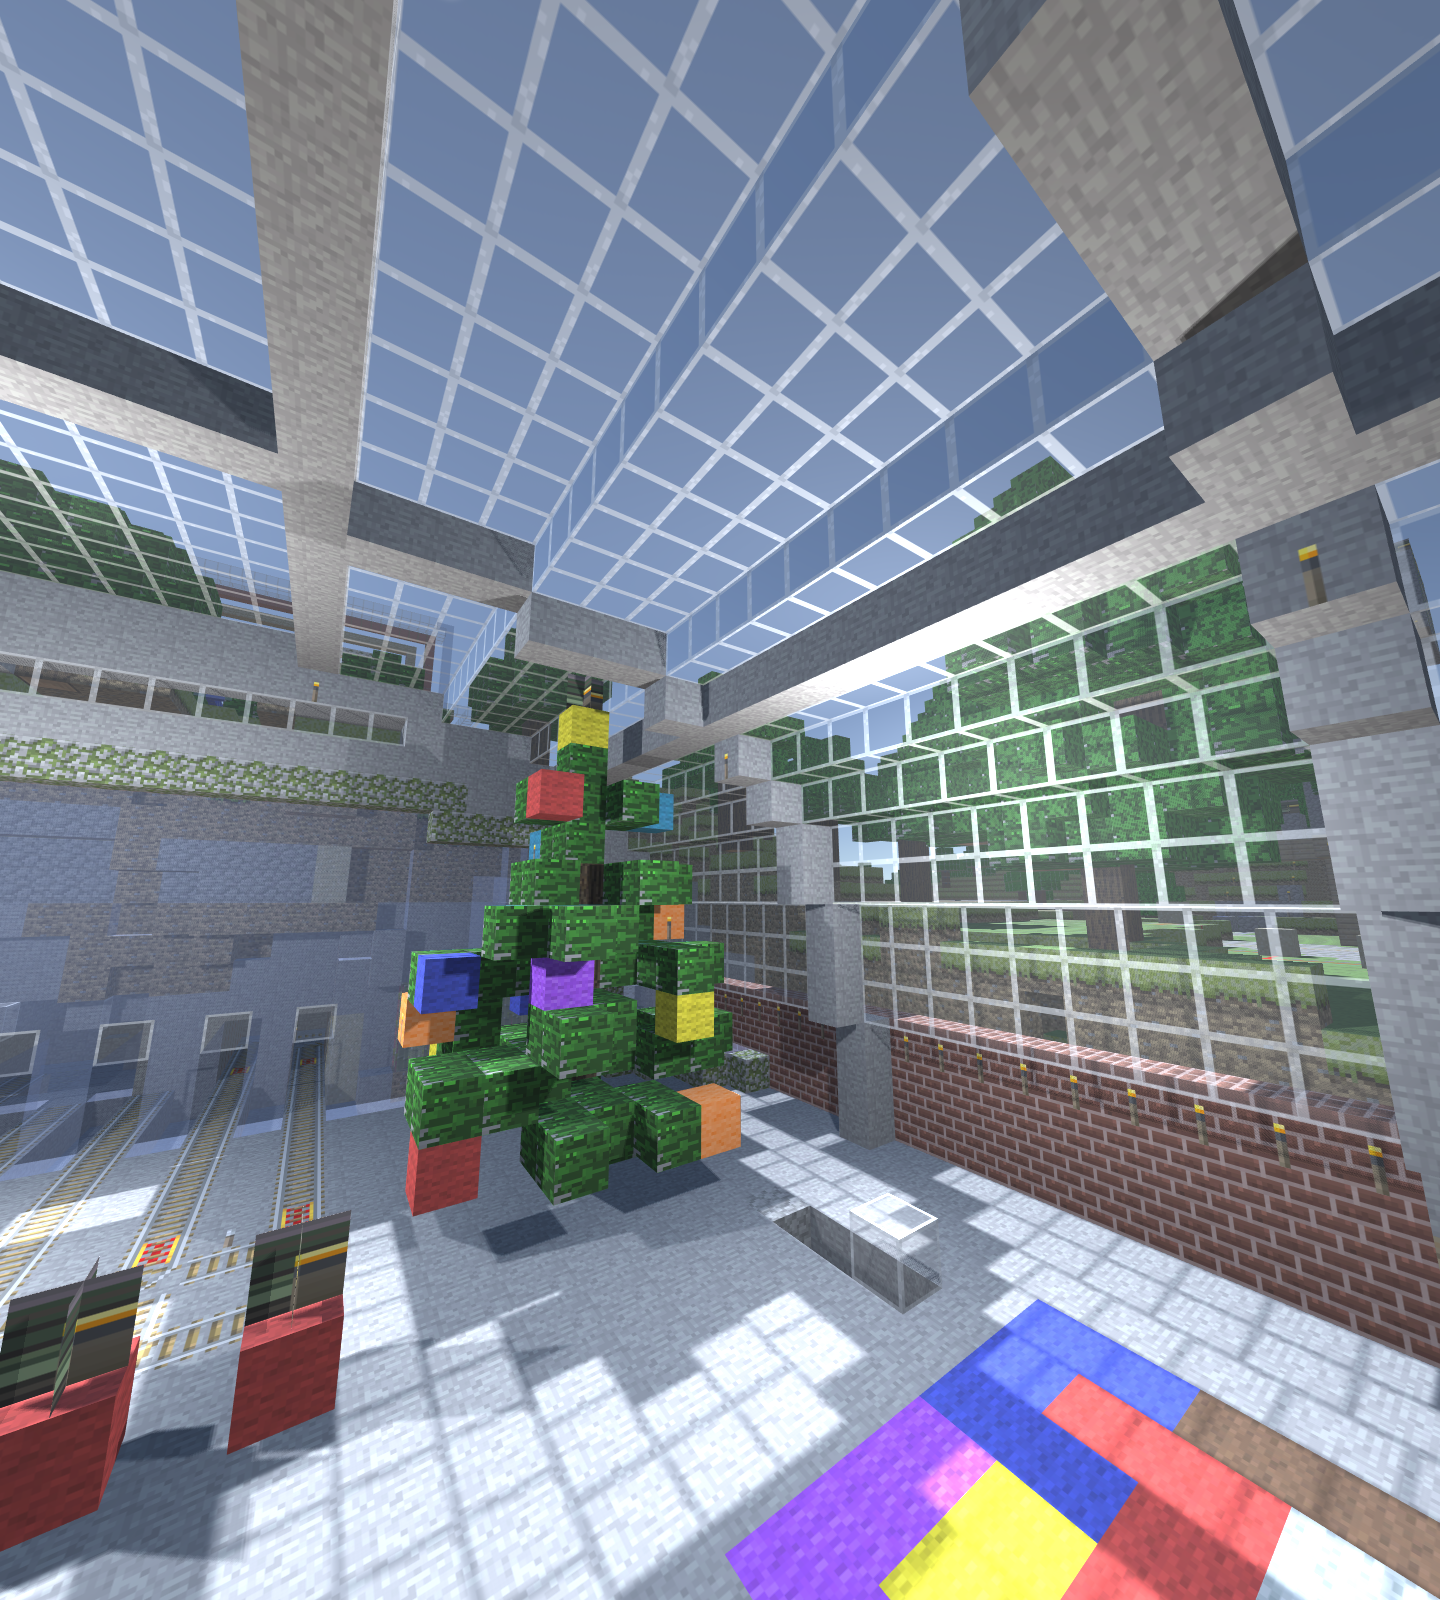
\includegraphics[width=0.96\linewidth]{TOG/figs/mc_gt3.png}}
        
        \subfloat[]{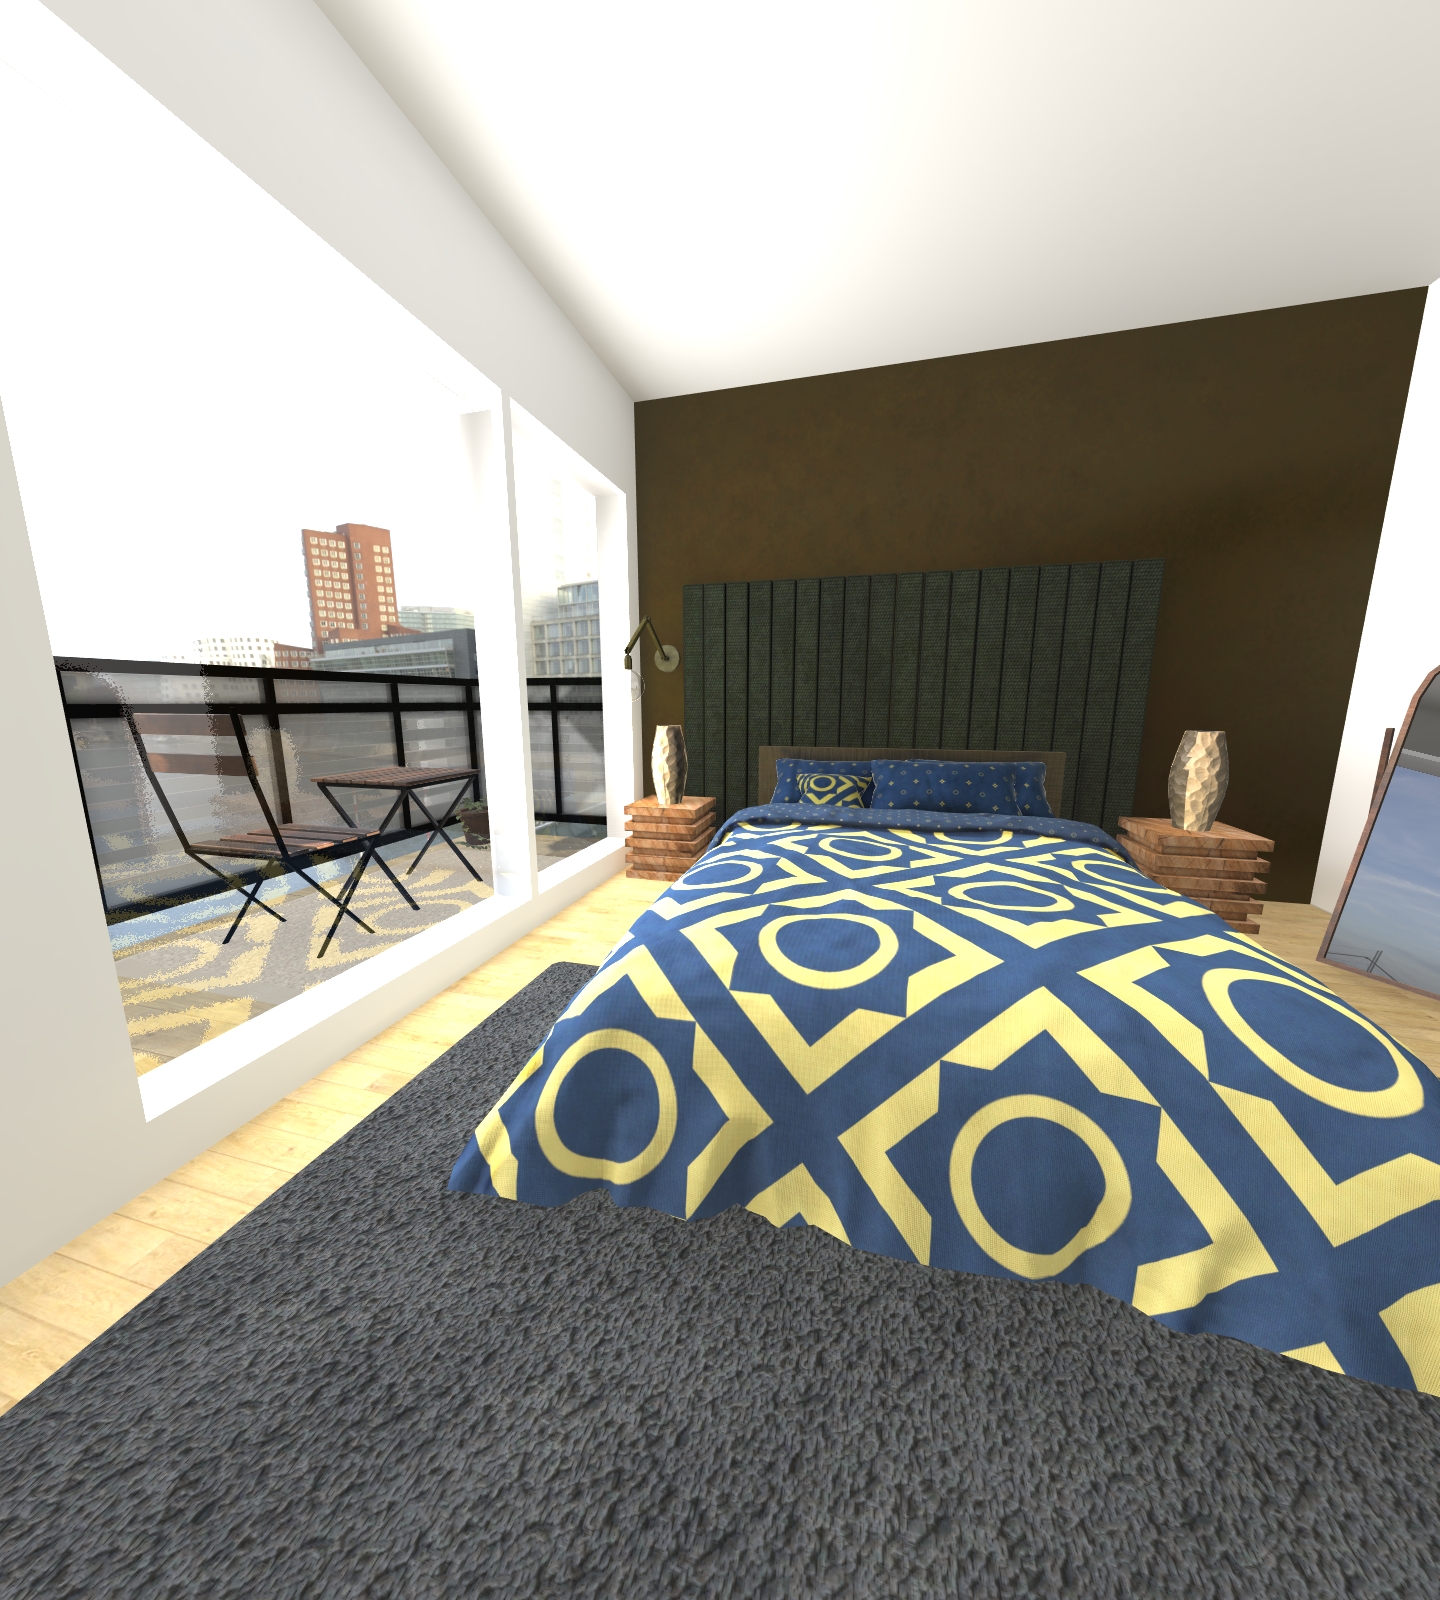
\includegraphics[width=0.96\linewidth]{TOG/figs/bed_gt0.png}}
    \end{minipage}
    \begin{minipage}{0.32\linewidth} %ours
        \subfloat[]{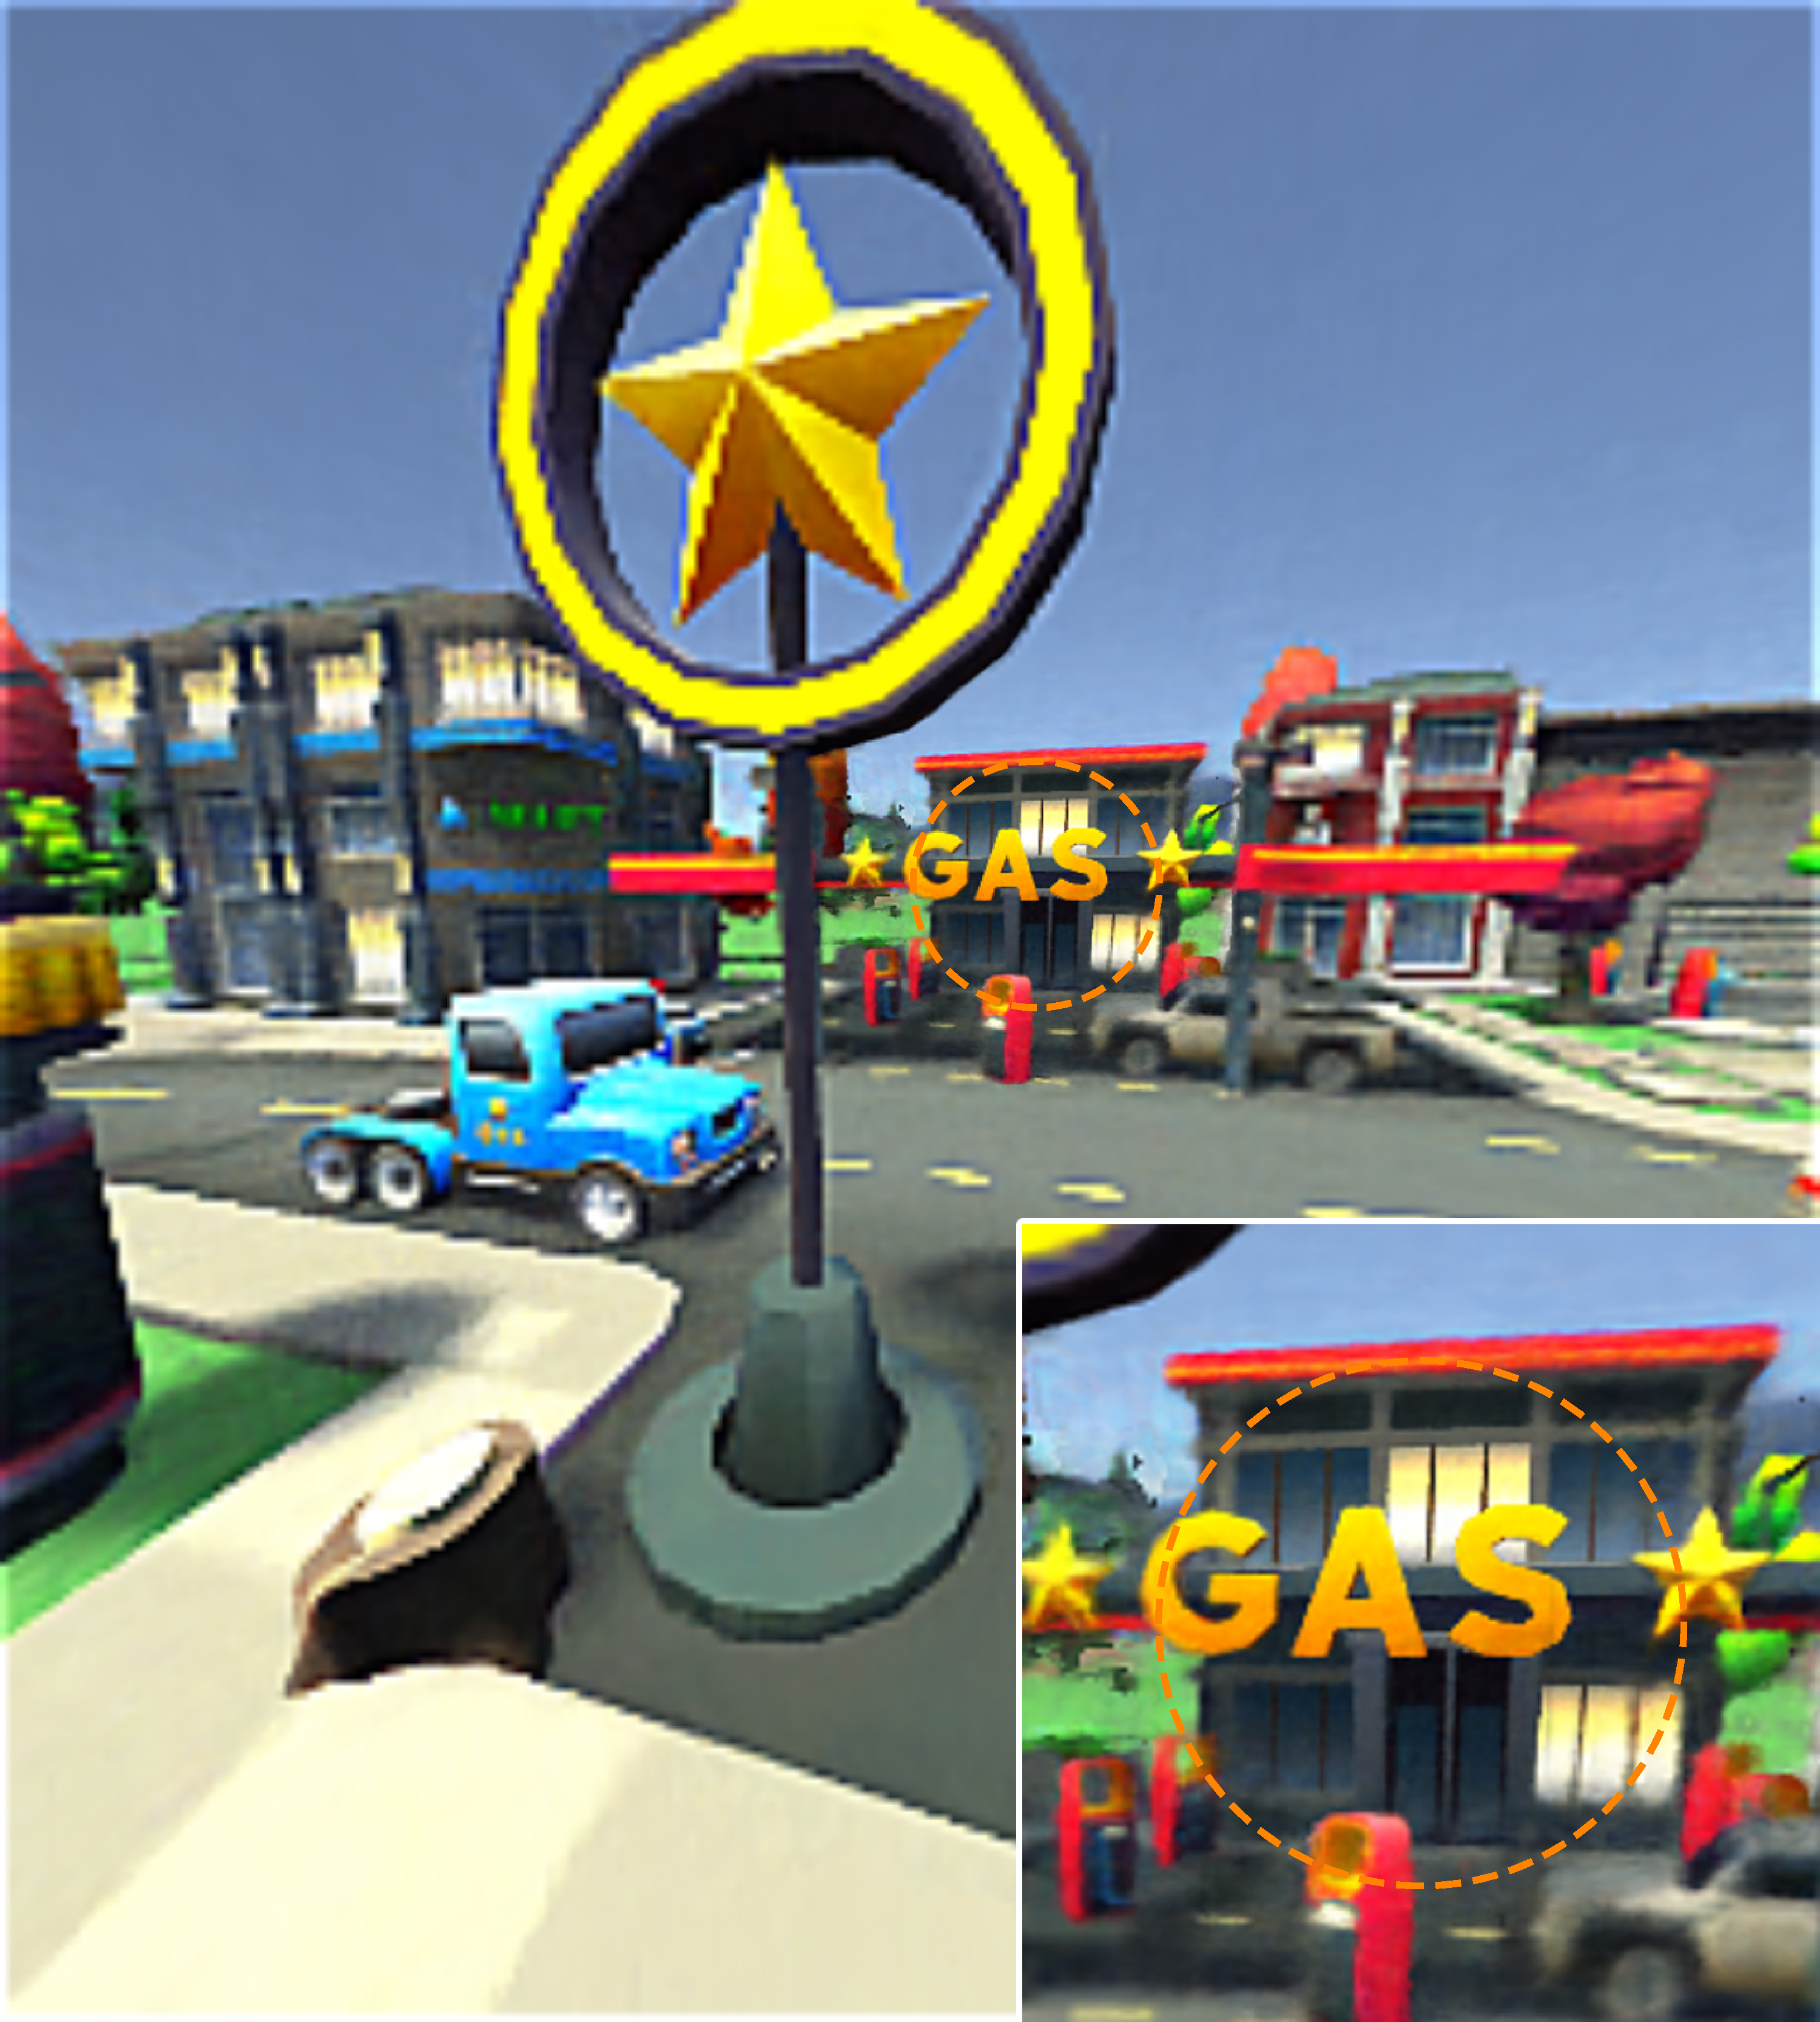
\includegraphics[width=0.96\linewidth]{TOG/figs/gas_our4_inset.pdf}}
        
        \subfloat[]{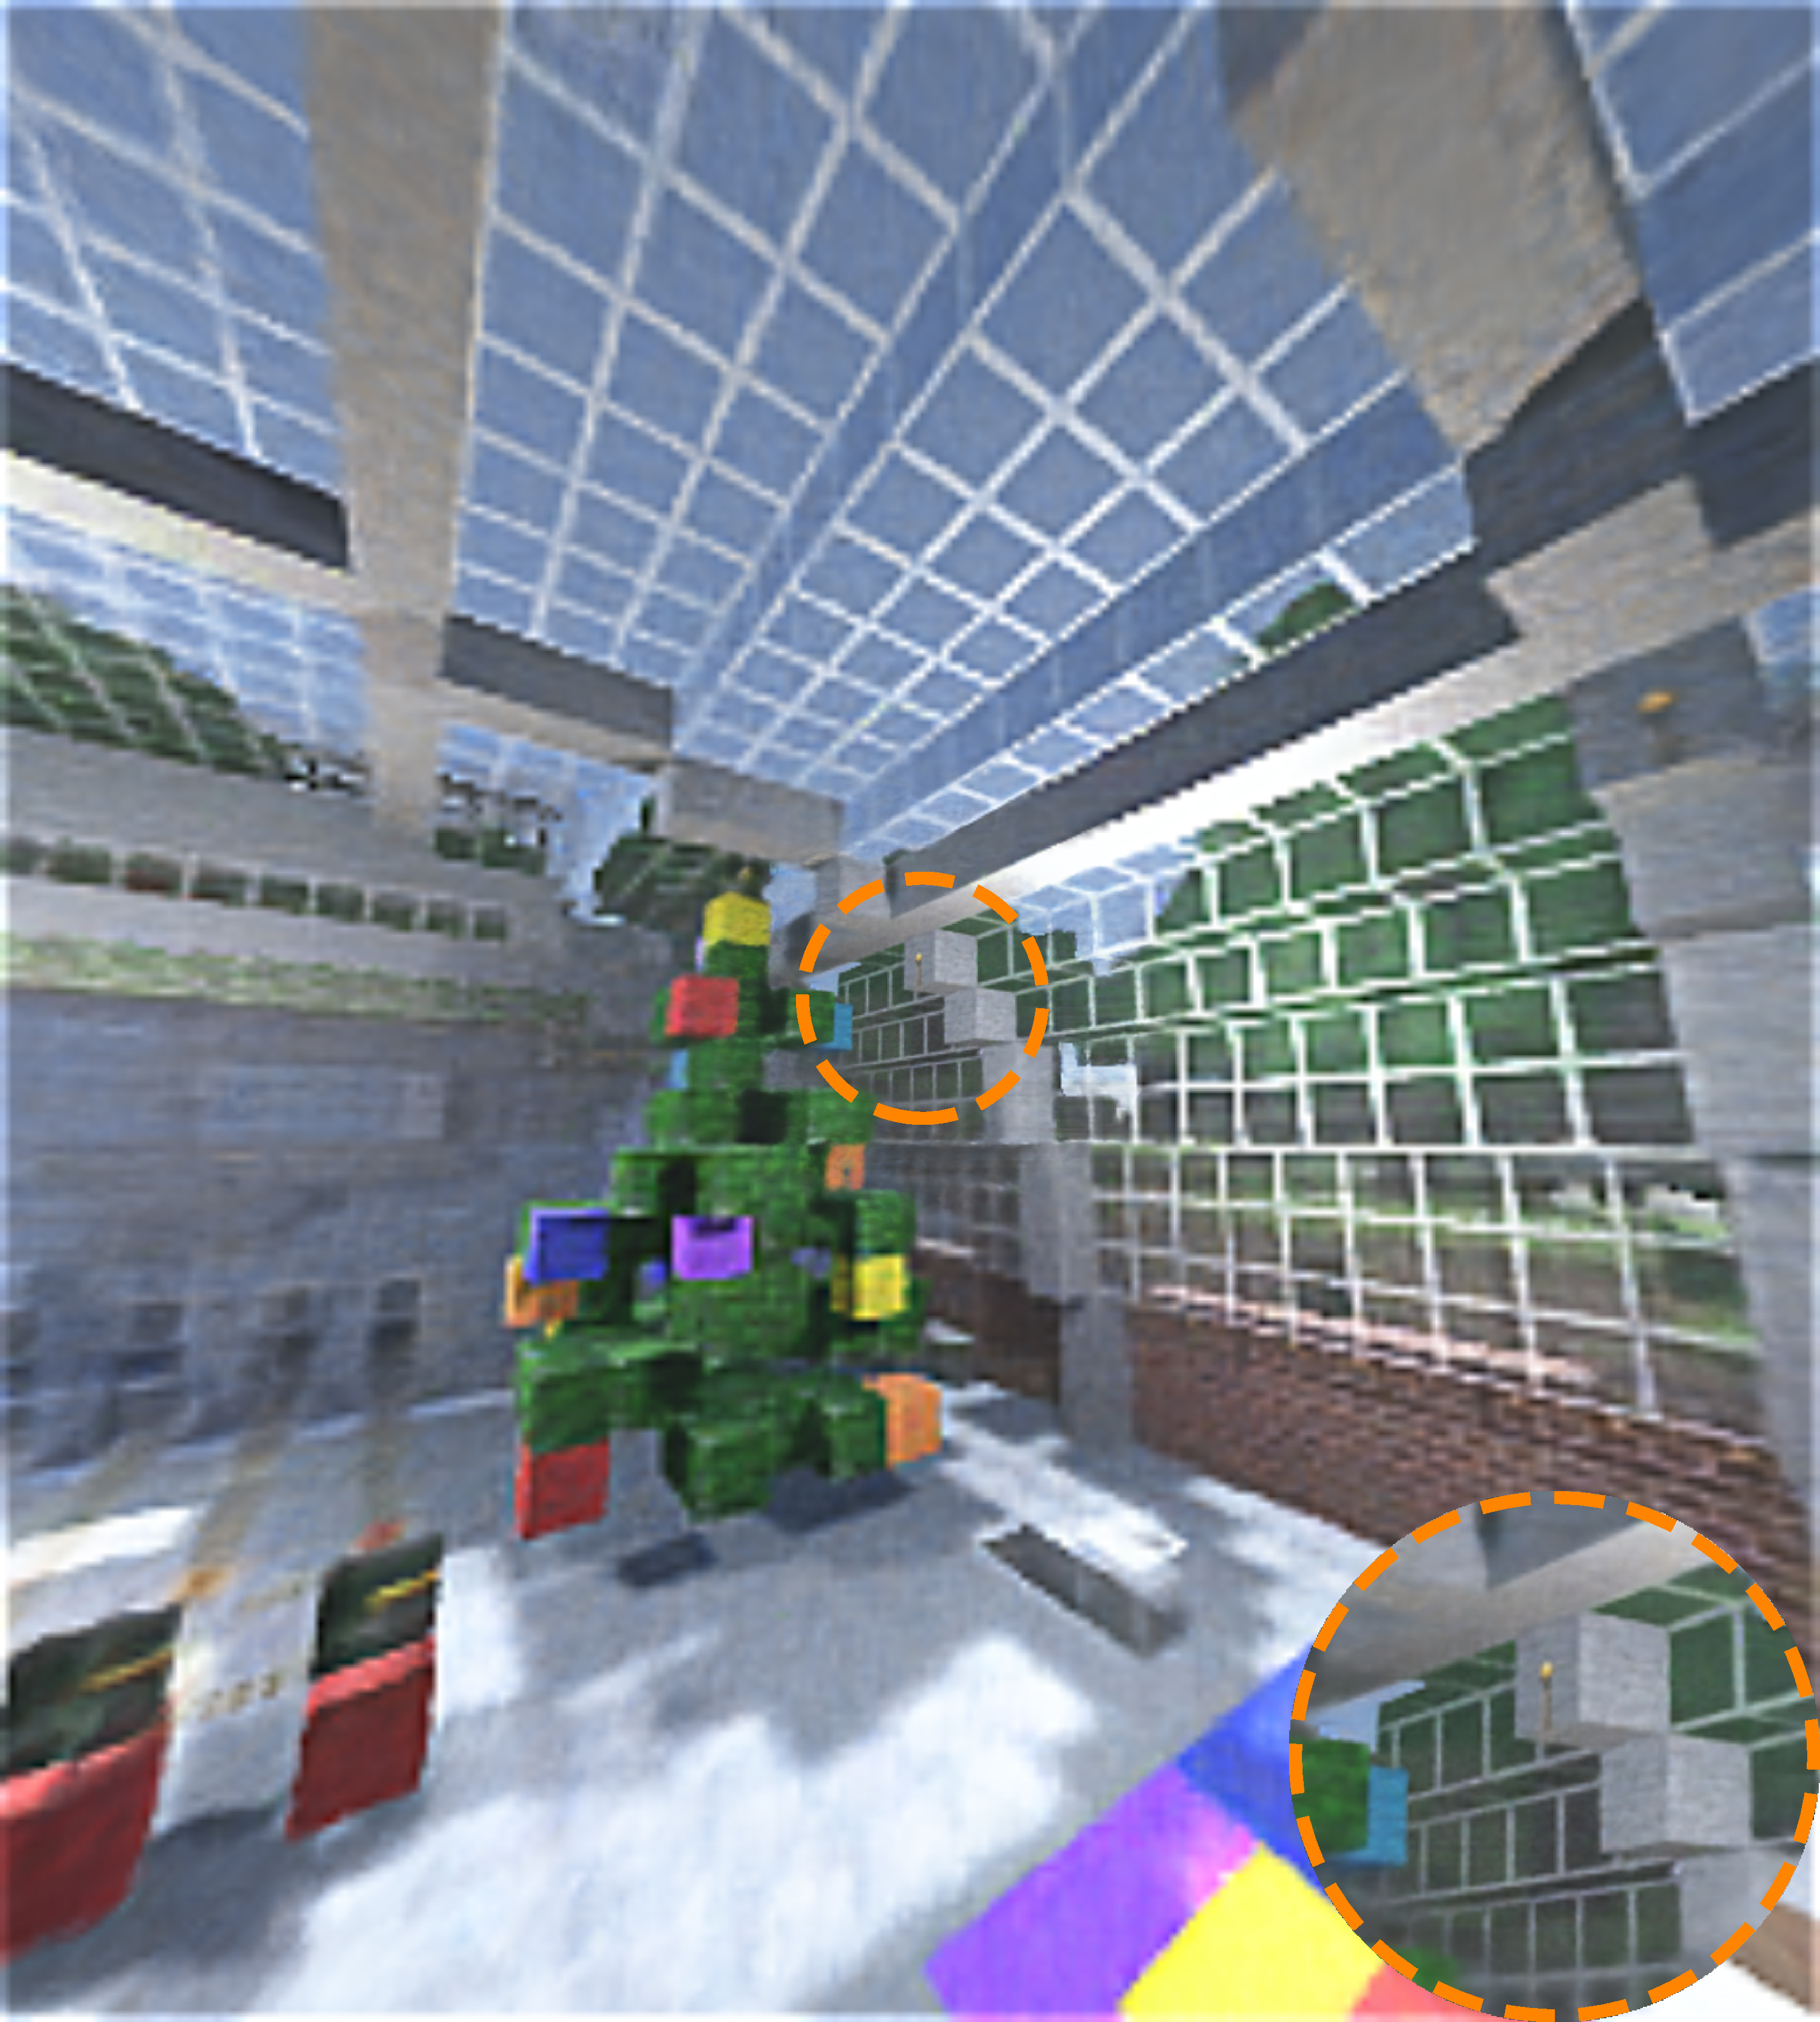
\includegraphics[width=0.96\linewidth]{TOG/figs/mc_our3_inset.pdf}}
        
        \subfloat[]{\includegraphics[width=0.96\linewidth]{example-image-a}}               
    \end{minipage}
    \begin{minipage}{0.32\linewidth} % NERF
        \subfloat[]{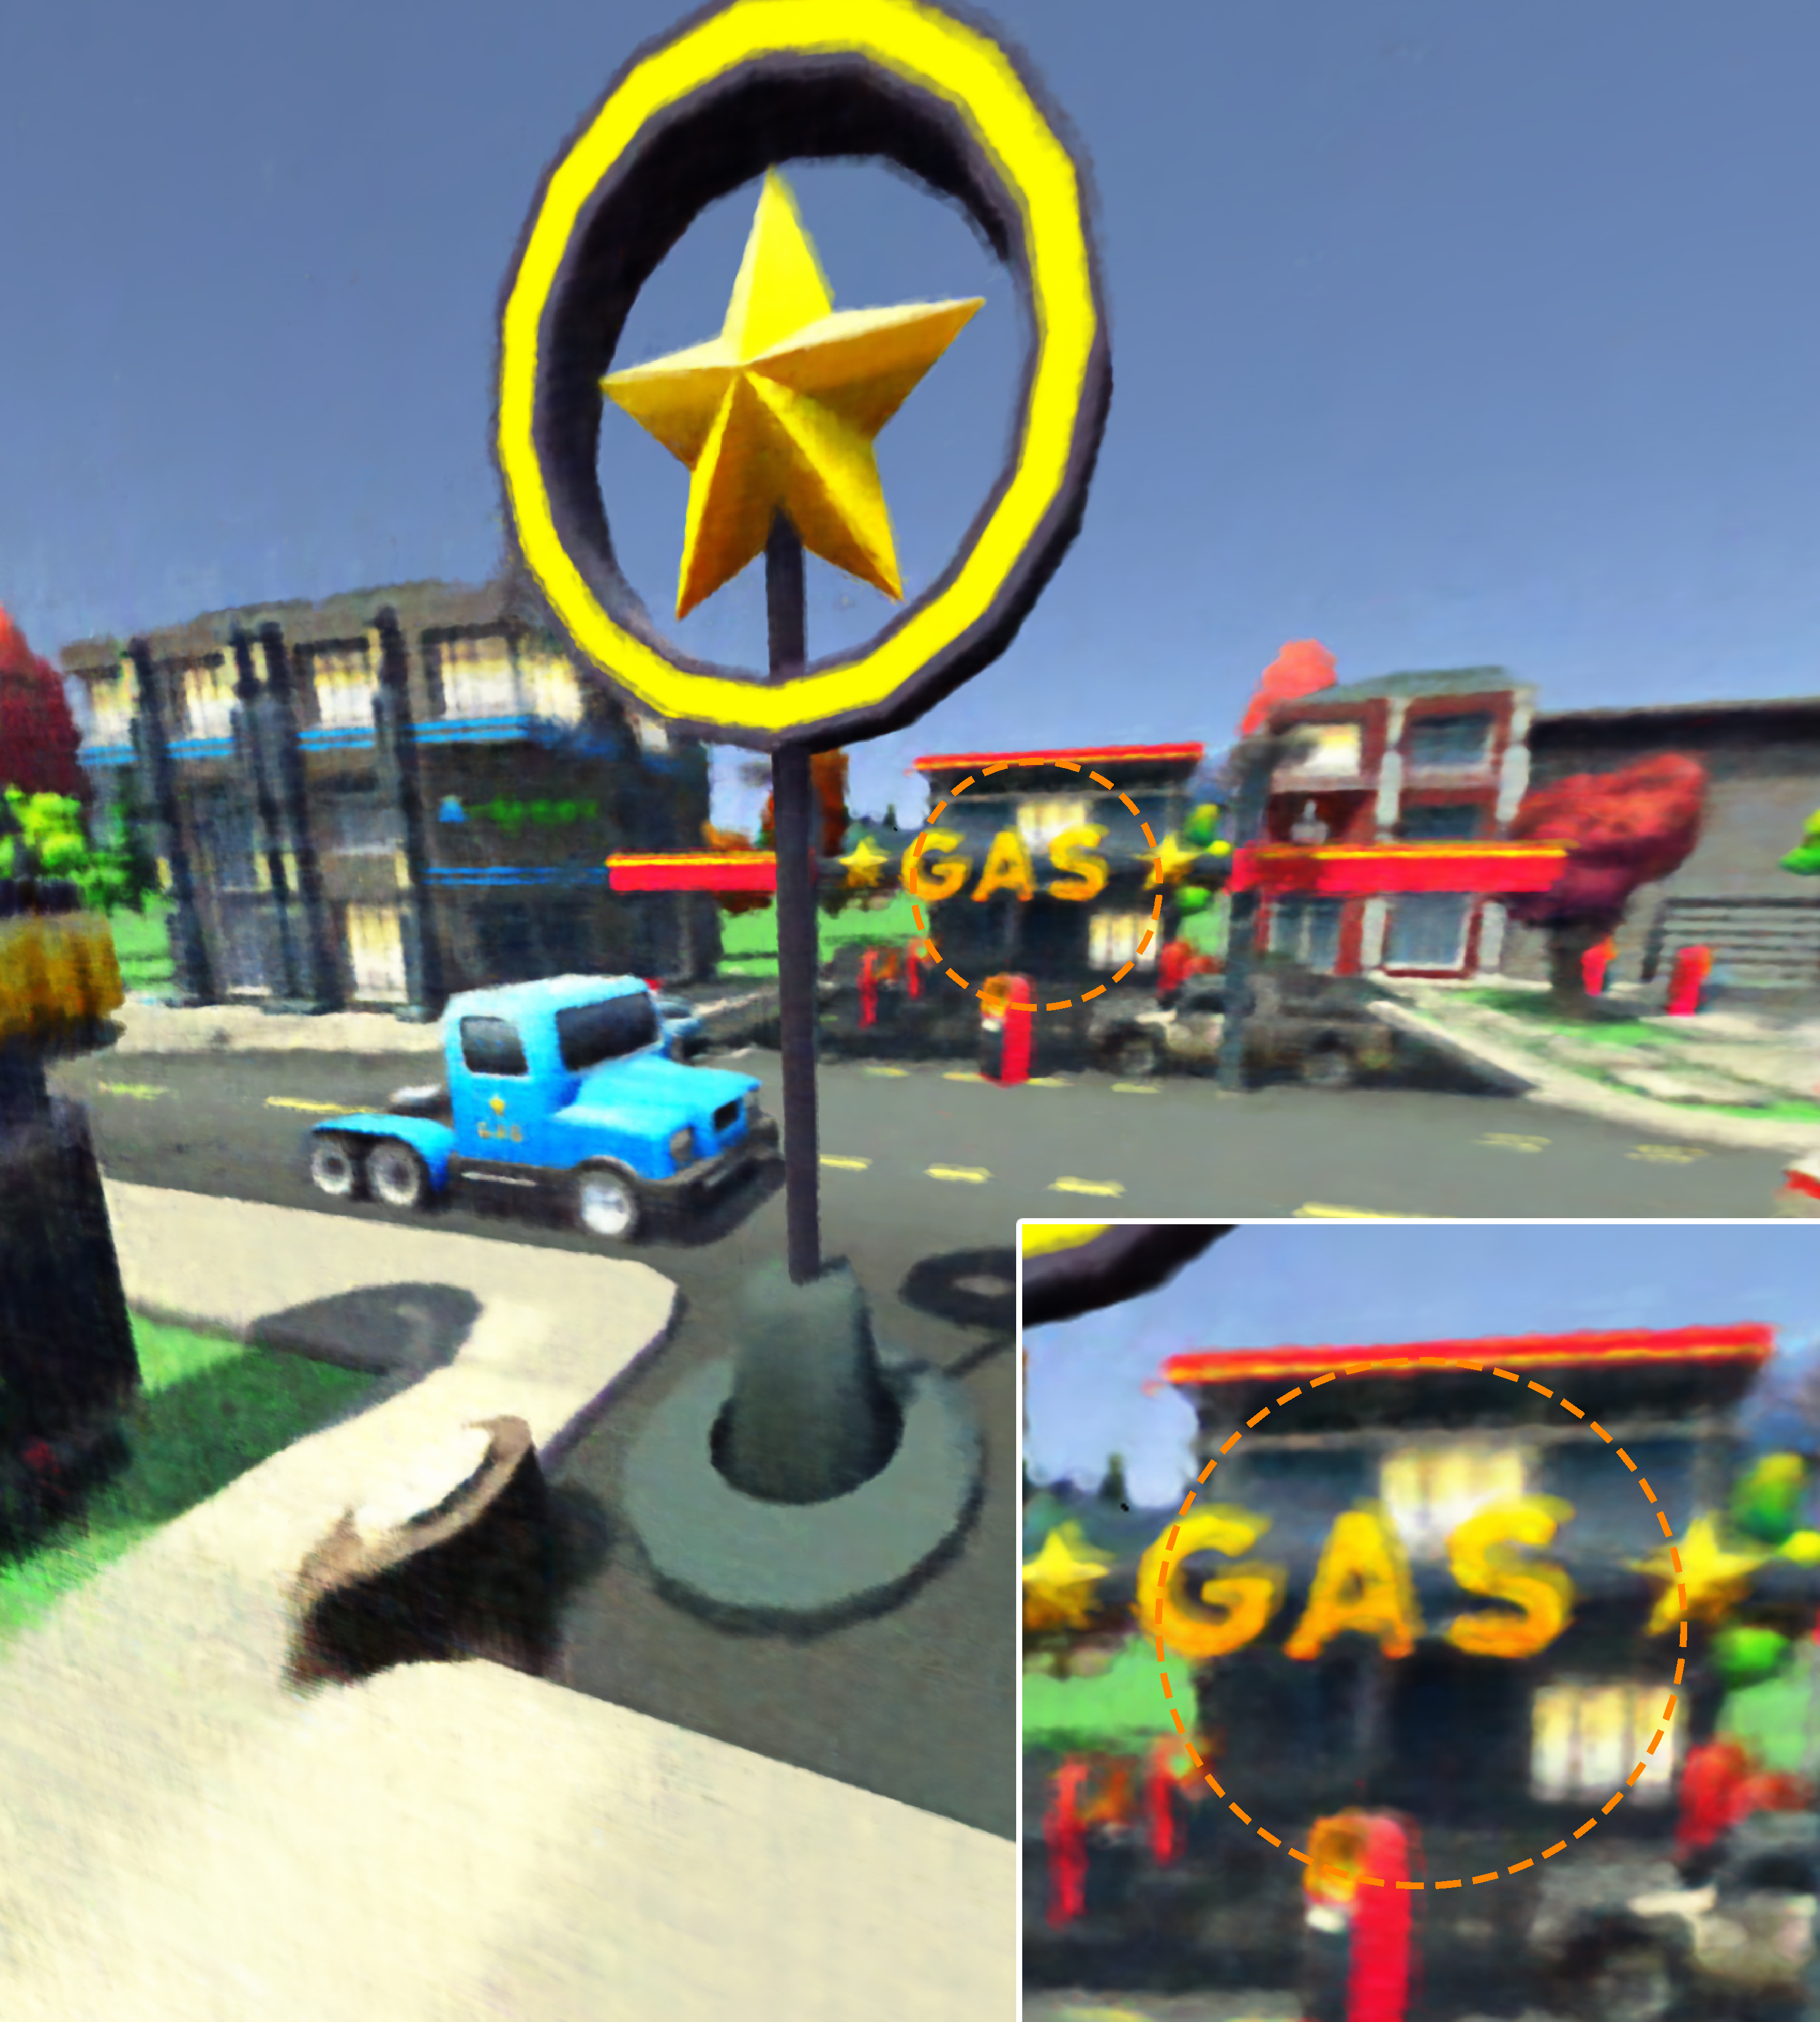
\includegraphics[width=0.96\linewidth]{TOG/figs/gas_nerf4_inset.pdf}}
        
        \subfloat[]{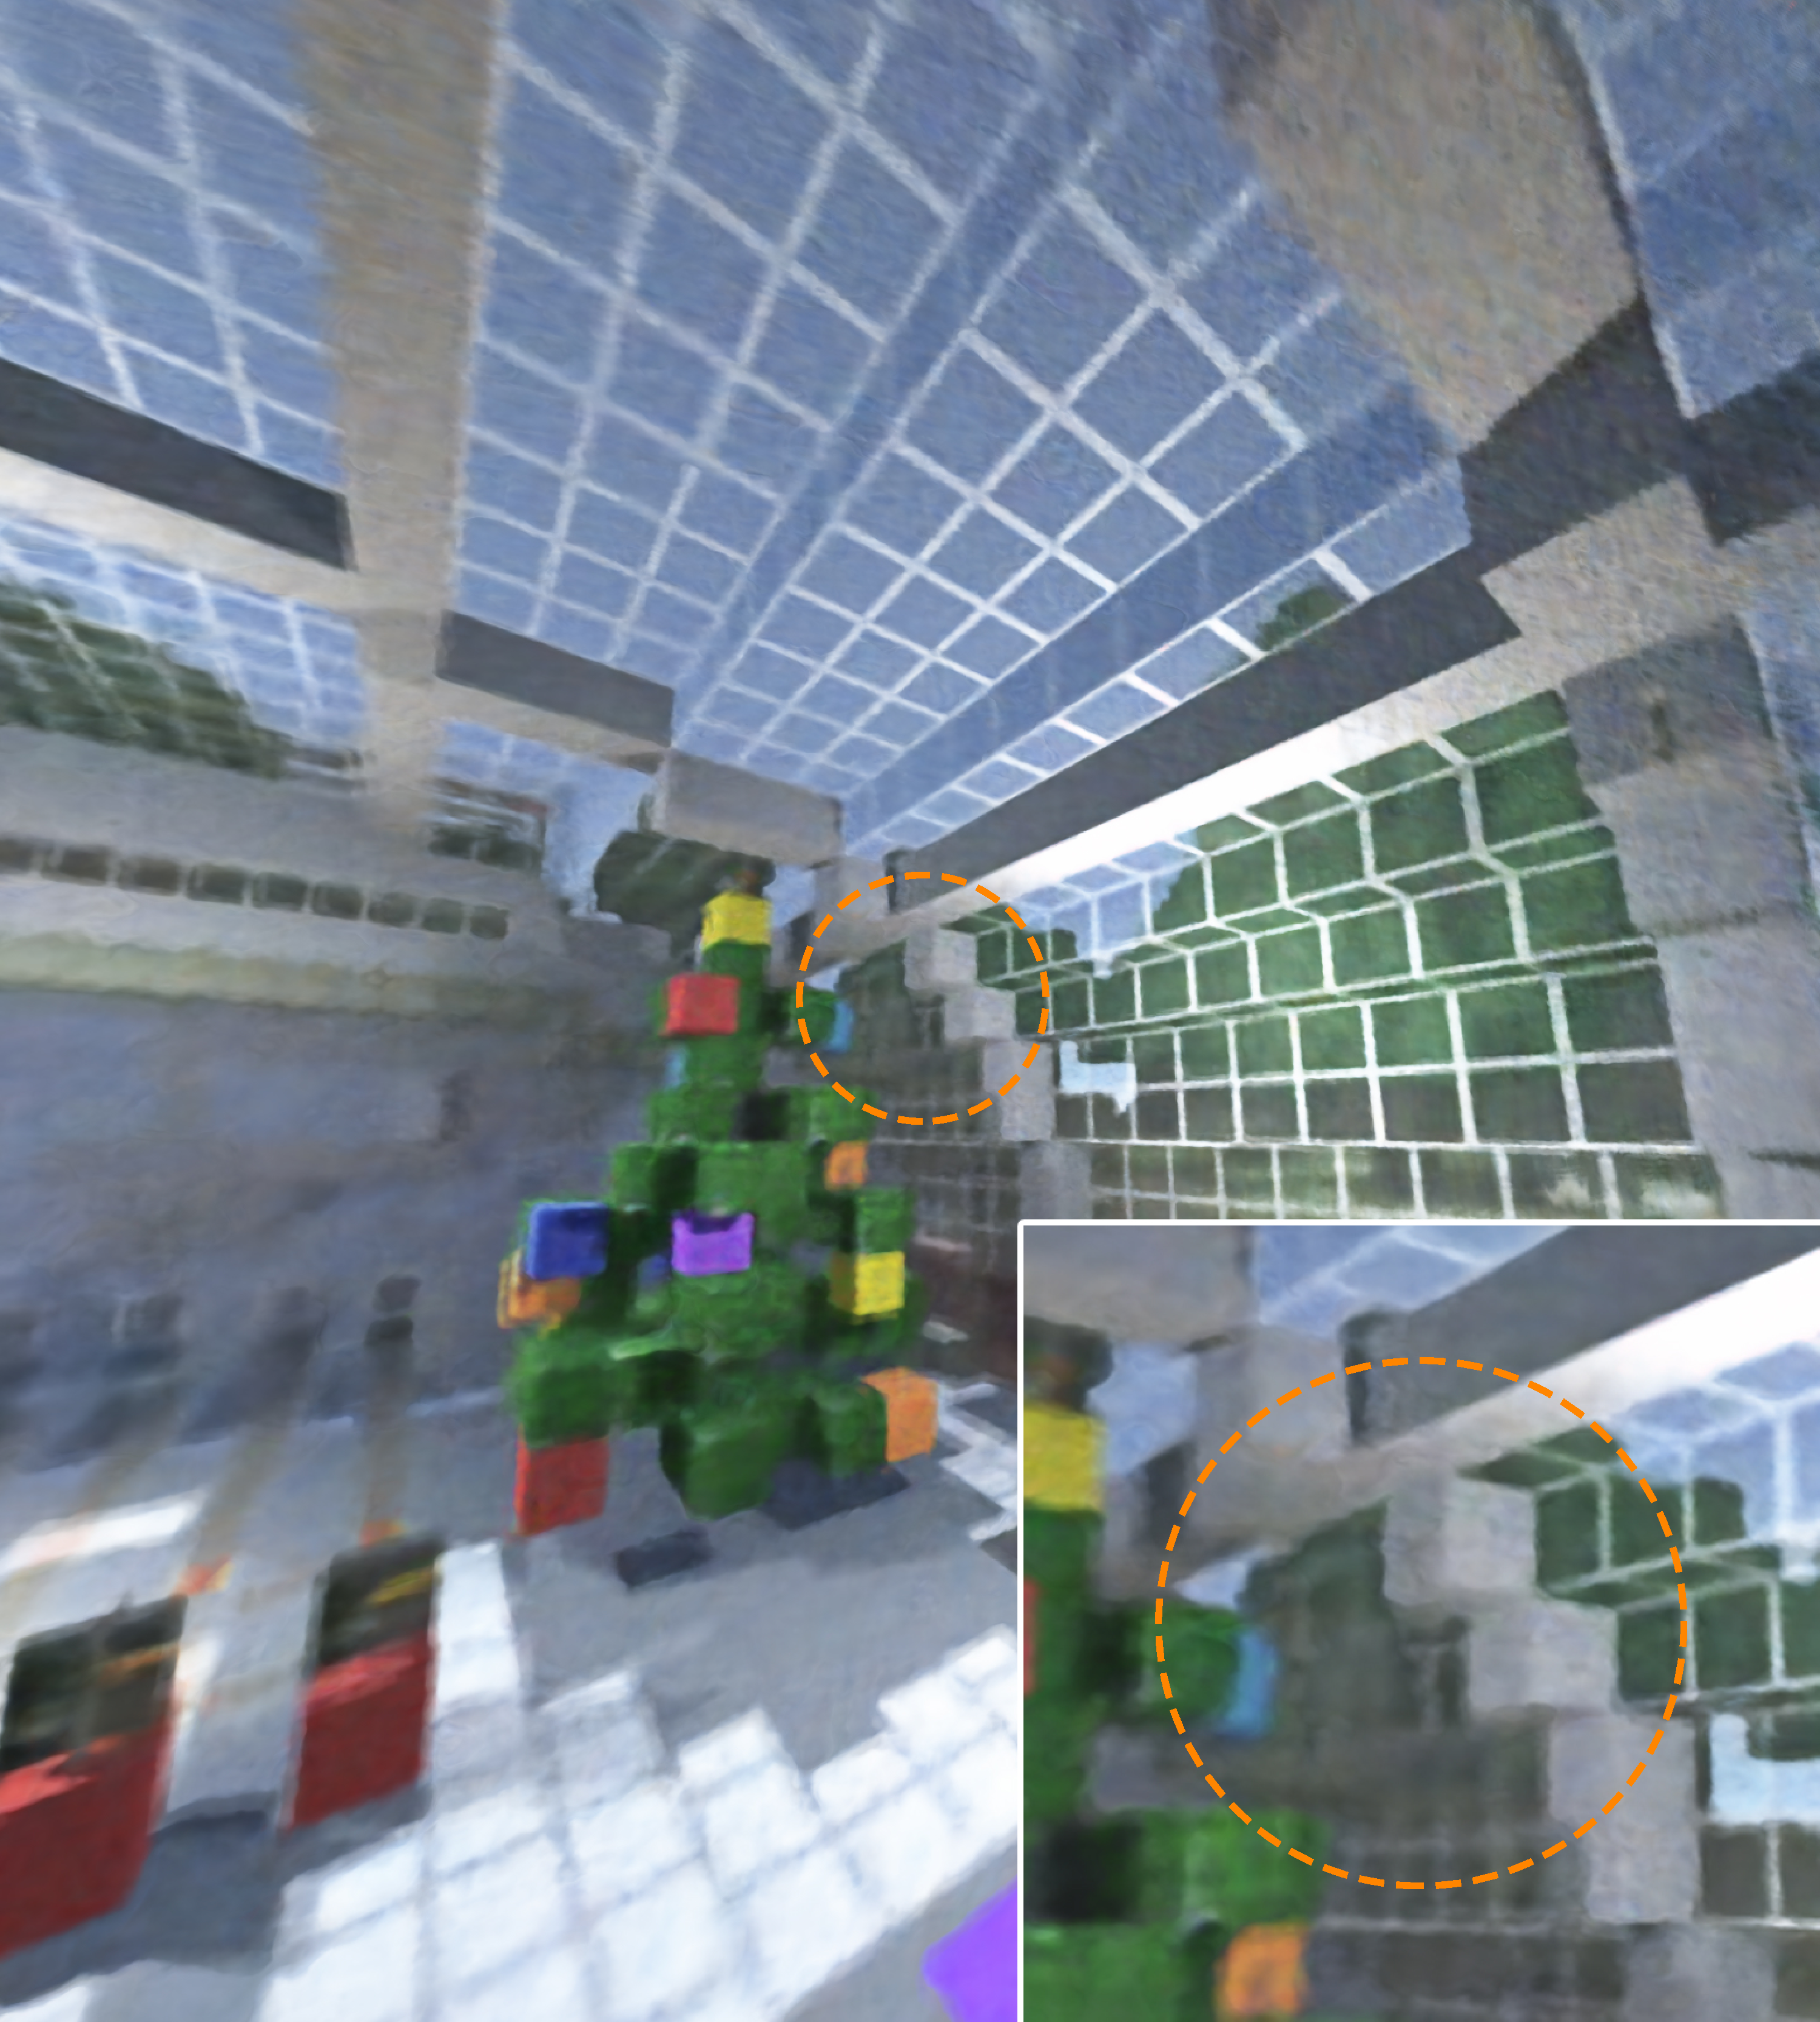
\includegraphics[width=0.96\linewidth]{TOG/figs/mc_nerf3_inset.pdf}}
        
        \subfloat[]{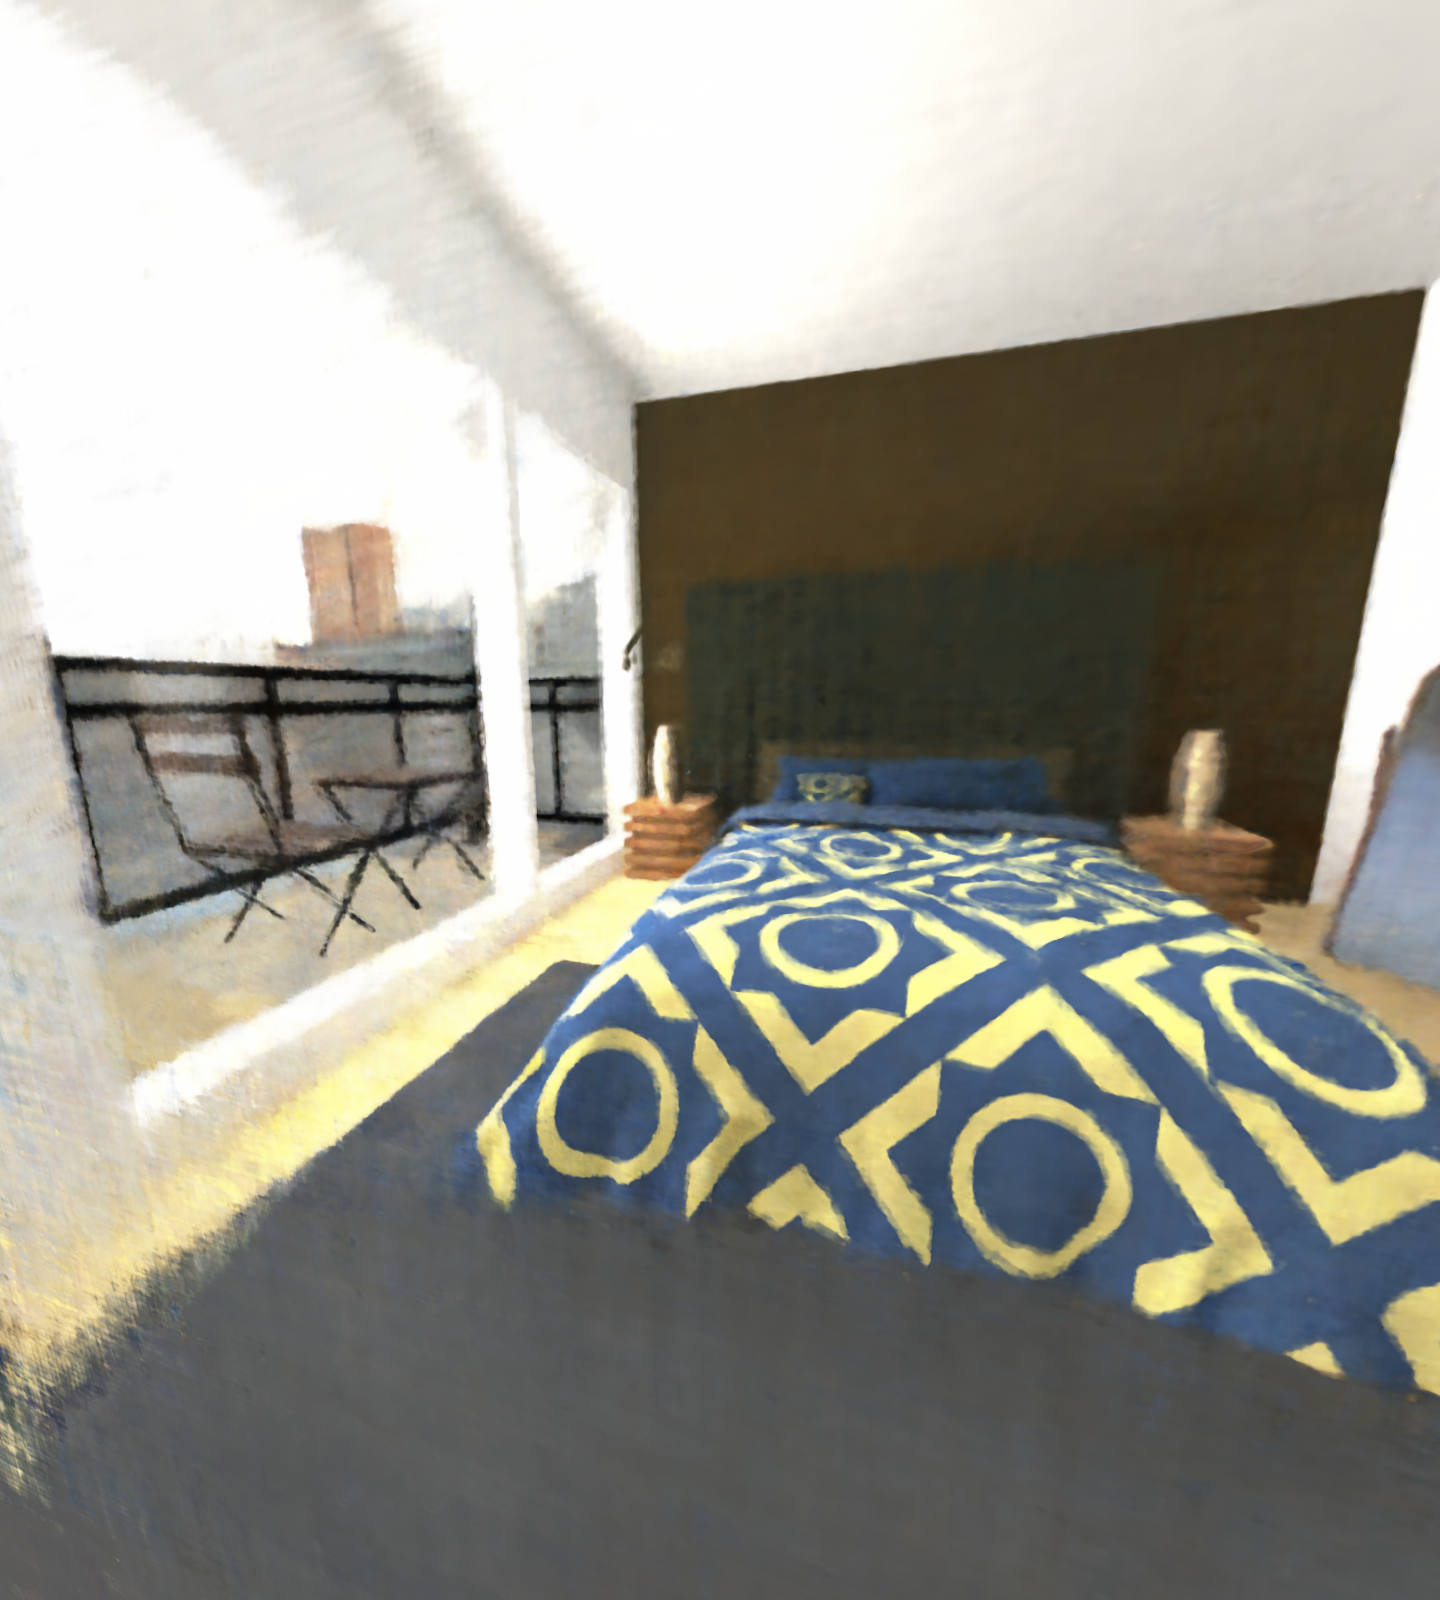
\includegraphics[width=0.96\linewidth]{TOG/figs/bed_nerf0.png}}      
    \end{minipage}    
    
    \caption{Comparing our synthesis method with full resolution (2nd column) rendering and NeRF (3rd column).}
    {\zh{add inset for 2nd and 3rd col}}
    \label{fig:results:comparison}
\end{figure*}

\begin{figure*}[htb]
    \centering
    \begin{minipage}{0.32\linewidth} %full res
        
        \subfloat[]{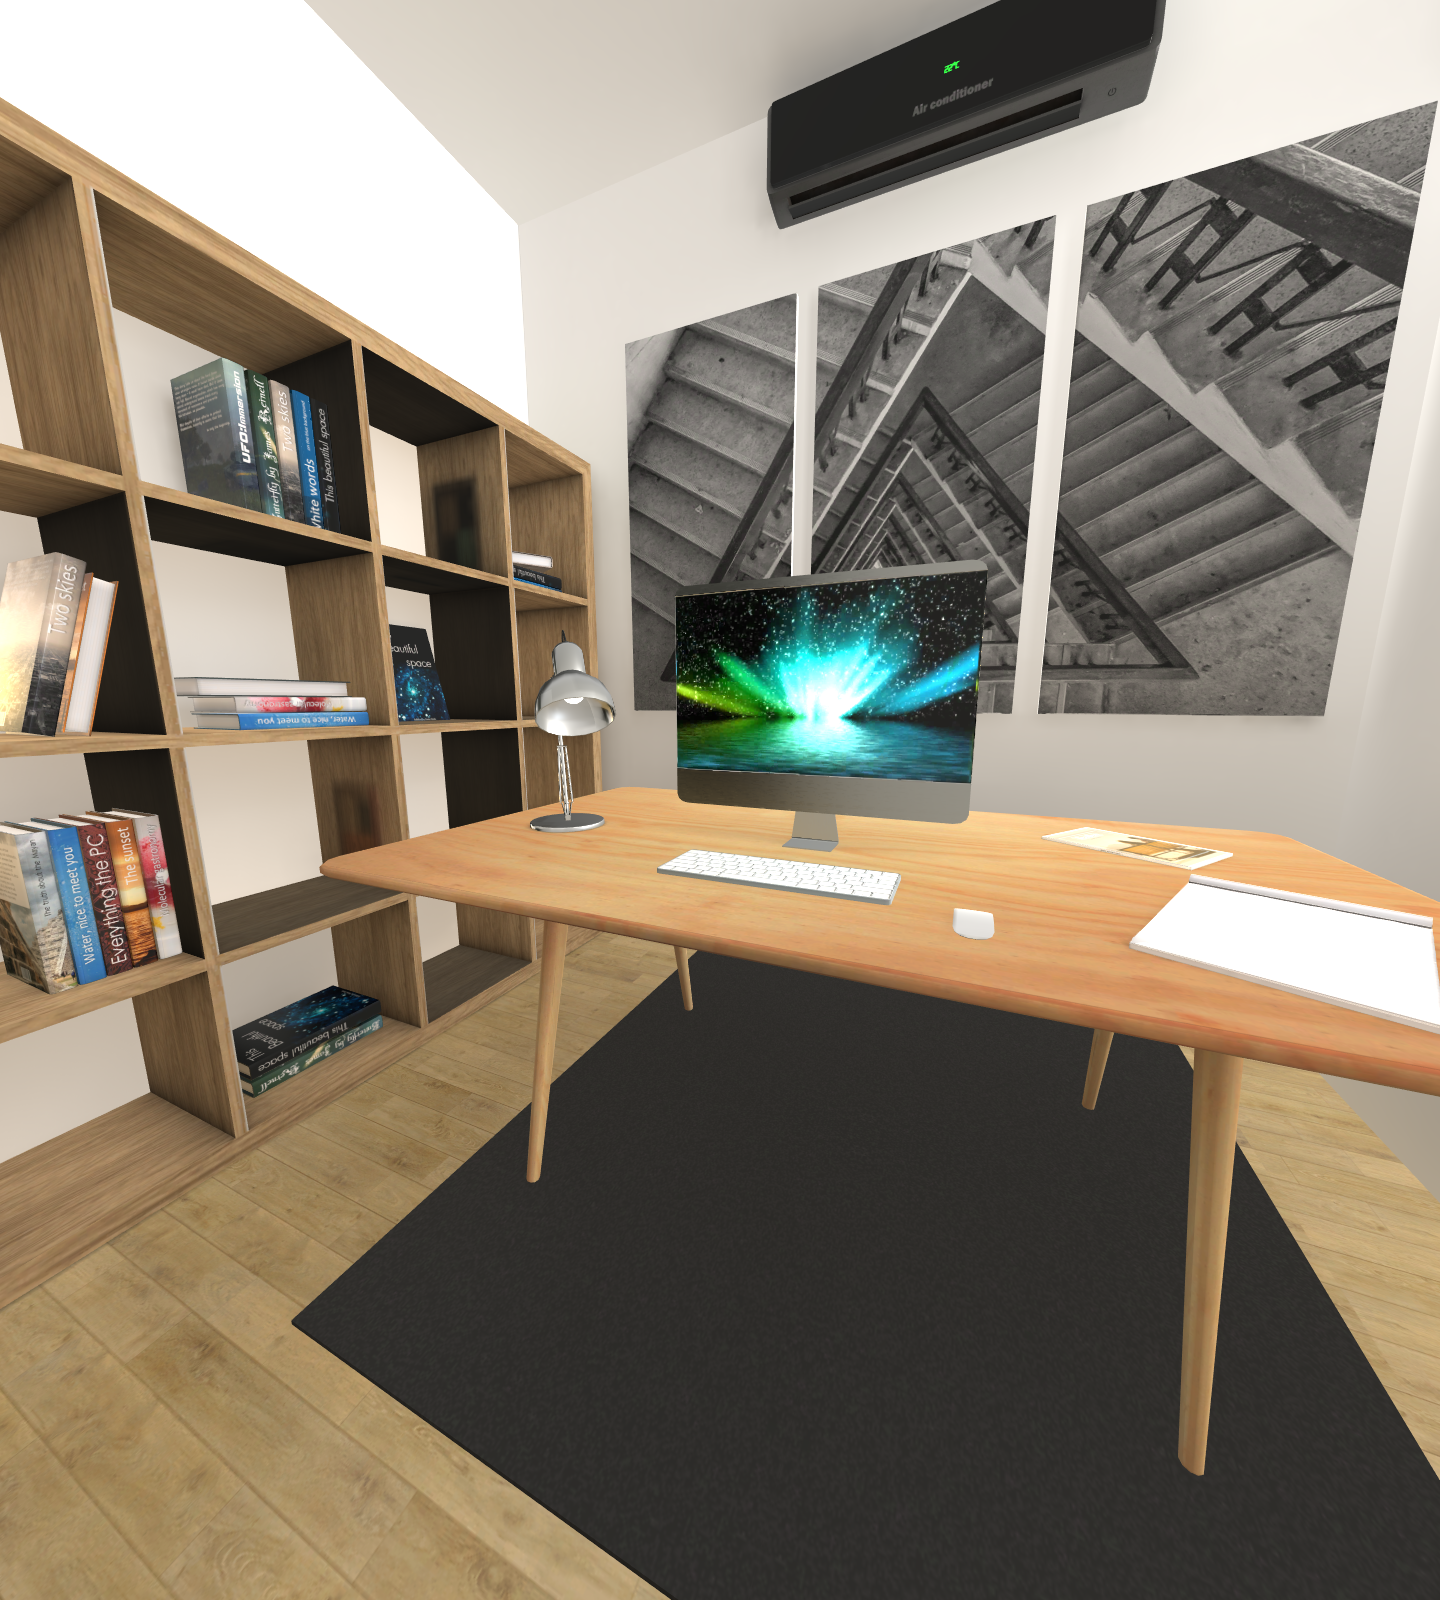
\includegraphics[width=0.96\linewidth]{TOG/figs/study_gt0.png}}
    \end{minipage}
    \begin{minipage}{0.32\linewidth} %ours
        
        \subfloat[]{\includegraphics[width=0.96\linewidth]{example-image-a}}                
    \end{minipage}
    \begin{minipage}{0.32\linewidth} % NERF
        
        \subfloat[]{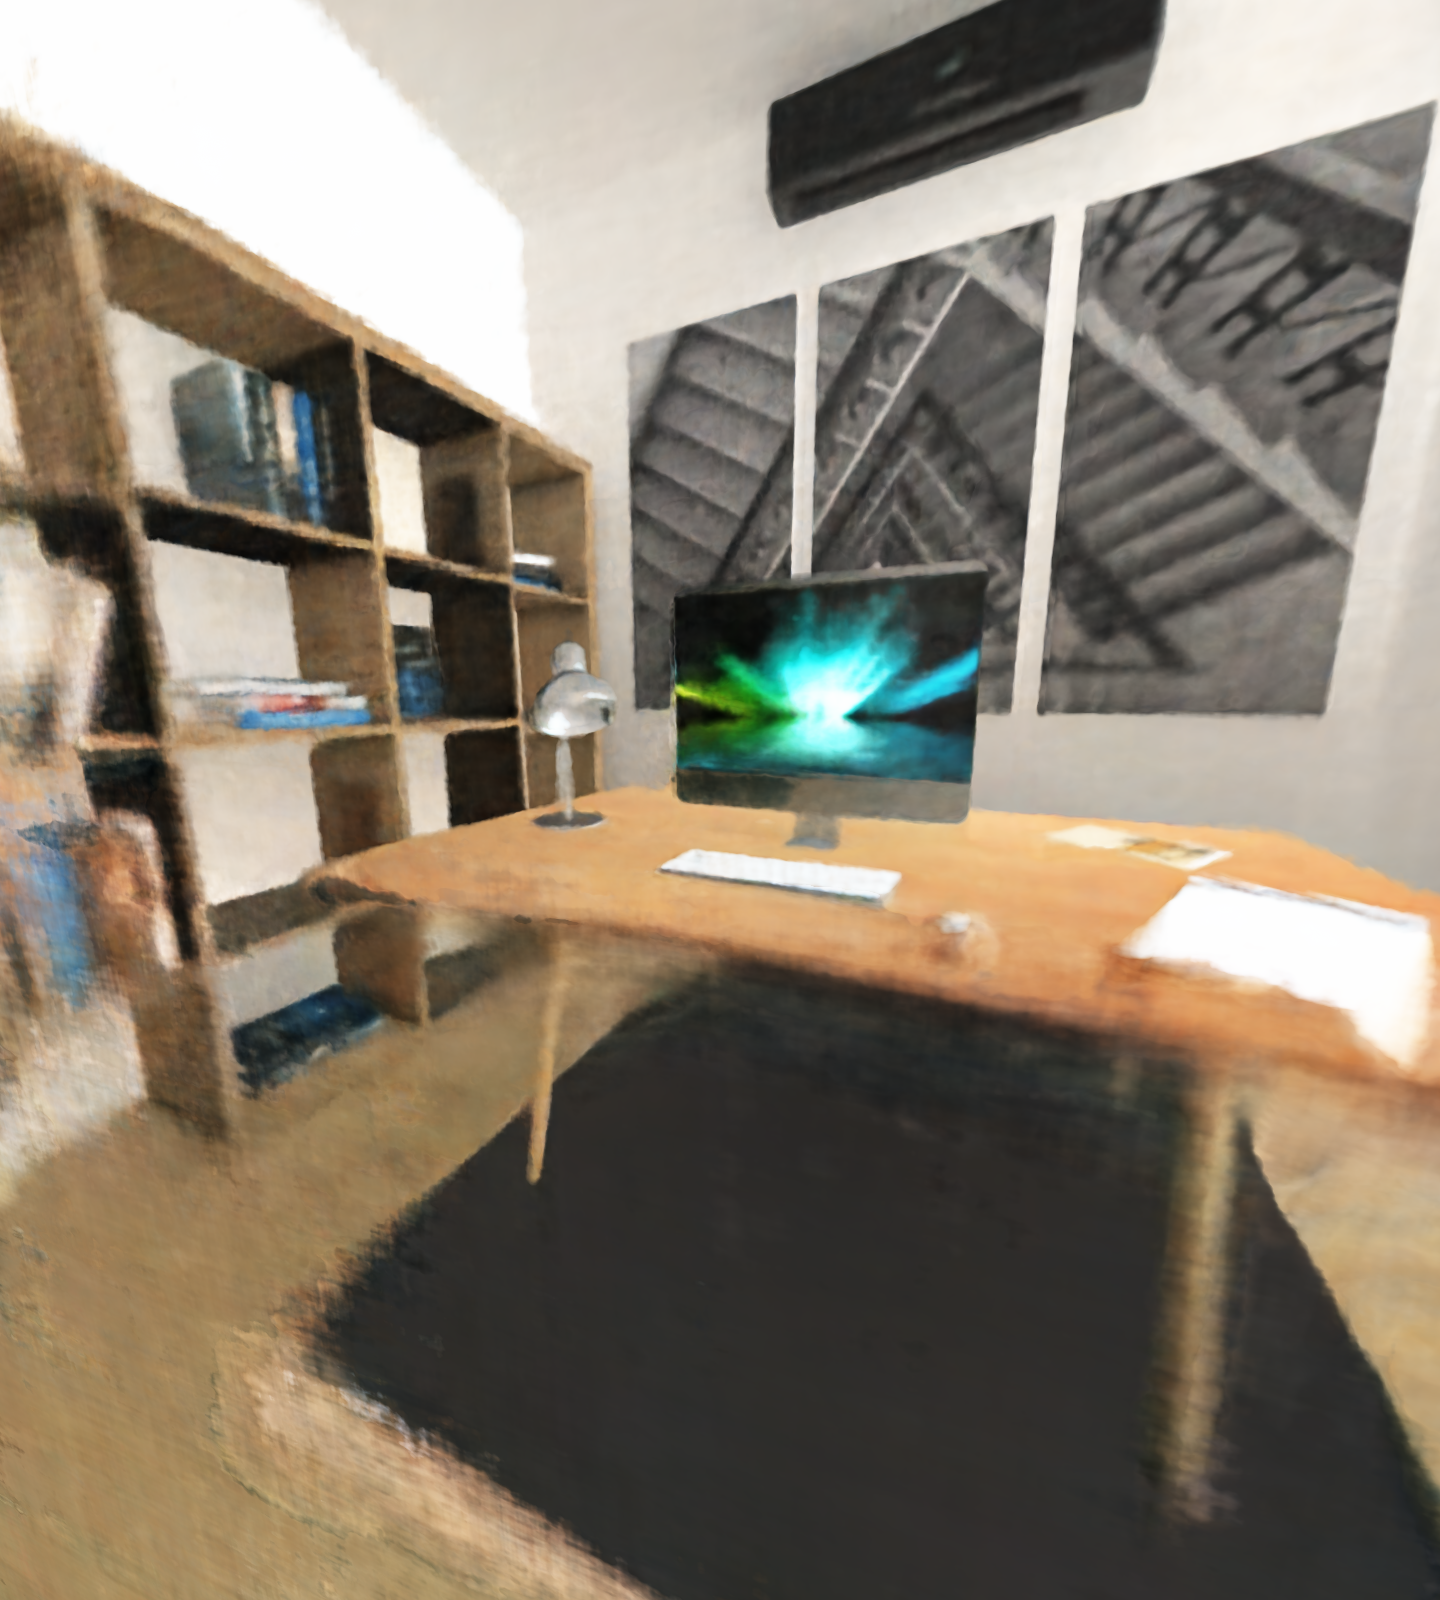
\includegraphics[width=0.96\linewidth]{TOG/figs/study_nerf0.png}}        
    \end{minipage}    
    
    \caption{Comparing our synthesis method with full resolution (2nd column) rendering and NeRF (3rd column) (Cont.).}
    {\zh{add inset for 2nd and 3rd col}}
    \label{fig:results:comparison2}
\end{figure*}


\subsection{Ablation Study}
% the performance of an AI system by removing certain components, to understand the contribution of the component to the overall system

\subsection{Spatial-Temporal Optimality}

% apply objective metric to Fig 7, aka different sample numbers
